\documentclass[11pt,letterpaper]{article}
\usepackage[lmargin=1in,rmargin=1in,bmargin=1in,tmargin=1in]{geometry}
\usepackage{../style}

\setlength{\parindent}{0ex}

% -------------------
% Content
% -------------------
\begin{document}

\pagenumbering{gobble}

% Recitation: Rational Functions
\phantom{} \hfill {\bfseries \Large Recitation: Rational Functions} \hfill \phantom{} \par\vspace{0.5cm}

% Problem 1
\noindent {\bfseries Problem 1.} Consider the rational function given below:
	\[
	f(x)= \dfrac{x^2 + 10x + 25}{x^2 + 8x + 15}
	\]
Complete the following parts:
	\begin{enumerate}[(a)]
	\item Find the domain.
	\item Find any $y$-intercepts.
	\item Find any $x$-intercepts.
	\item Find any vertical asymptotes. 
	\item Find any horizontal asymptotes.
	\item Find any holes.
	\end{enumerate} \vfill



% Problem 2
\noindent {\bfseries Problem 2.} Consider the rational function given below:
	\[
	g(x)= \dfrac{2x^3 + x^2 - x}{x^3 + 2x^2 - 3x}
	\]
Complete the following parts:
	\begin{enumerate}[(a)]
	\item Find the domain.
	\item Find any $y$-intercepts.
	\item Find any $x$-intercepts.
	\item Find any vertical asymptotes. 
	\item Find any horizontal asymptotes.
	\item Find any holes.
	\end{enumerate} \vfill



\newpage



% Problem 3
\noindent {\bfseries Problem 3.} For each of the following, find a rational function with the given properties: 
	\begin{enumerate}[(a)]
	\item A function with domain $(-\infty, 5) \cup (5, \infty)$ and a root at $x= 2$.
	\item A function with a vertical asymptote at $x= 4$ and horizontal asymptote $y= 3$.
	\item A function with no $y$-intercept.
	\item A function with a hole at $(1, -2)$.
	\end{enumerate} \par\vspace{8cm}



% Problem 4
\noindent {\bfseries Problem 4.} Use the plot below to sketch the graph of $f(x)= \dfrac{x^2 - x - 2}{x^2 - 2x - 3}$. \par
	\[
	\fbox{
	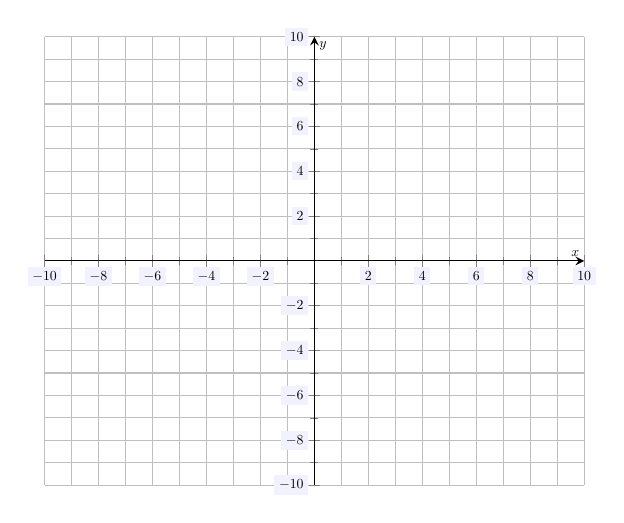
\begin{tikzpicture}[scale=1,every node/.style={scale=0.5}]
	\begin{axis}[
	grid=both,
	axis lines=middle,
	ticklabel style={fill=blue!5!white},
	xmin= -10, xmax=10,
	ymin= -10, ymax=10,
	xtick={-10,-8,...,10},
	ytick={-10,-8,...,10},
	minor x tick num = 1,
	minor y tick num = 1,
	xlabel=\(x\),ylabel=\(y\),
	]
%	\node at (11,6.6) {\Large$G(t)$};
%	\addplot[domain=0:22,samples=2,line width=0.03cm] (x, -0.5283*x+11.6);
	\end{axis}
	\end{tikzpicture}
	}
	\]

\end{document}